\documentclass{article}
\usepackage[accepted]{icml2018}
\usepackage{graphicx}

\icmltitlerunning{Neural Network Pruning Techniques}

\begin{document}

\twocolumn[
\icmltitle{E0:270 - Machine Learning - Neural Network Pruning Techniques}

\icmlsetsymbol{equal}{*}

\begin{icmlauthorlist}
\icmlauthor{Braunstein, Cameron}{dep2}
\icmlauthor{Nair, Abhishek}{dep1}
\icmlauthor{Shaw, Vishal}{dep3}
\end{icmlauthorlist}

\icmlaffiliation{dep1}{Department of Electronic System Engineering, Indian Institute of Science, Bangalore}
\icmlaffiliation{dep2}{Mathematics Department, Indian Institute of Science, Bangalore}
\icmlaffiliation{dep3}{Electrical Communication Engineering, Indian Institute of Science, Bangalore}

\icmlcorrespondingauthor{Braunstein, Cameron}{comeronb@iisc.ac.in}
\icmlcorrespondingauthor{Nair, Abhishek}{abhisheknair@iisc.ac.in}
\icmlcorrespondingauthor{Shaw, Vishal}{vishalshaw@iisc.ac.in}

\icmlkeywords{neural network, pruning, machine learning}

\vskip 0.3in
]

\printAffiliationsAndNotice{}

\begin{abstract}
This project investigated various methods of pruning a neural network. We have demonstrated the effectiveness of the L-OBS algorithm. While the N2PS algorithm may be effective on smaller networks, it does not scale up successfully. 
\end{abstract}

\section{Motivation}
\label{Motivation}
Deep neural networks are flexible function approximators that have been very successful in a
broad range of tasks. They can easily scale to millions of parameters, which results in challenges to store and load the network. Additionally, large networks have the problem of overfitting and can even memorize random patterns.(put citation). One of the methods that we investigate is to address these issues is neural network pruning, which seeks to remove unimportant weights from the network. This makes the networks smaller in memory and can reduce overfitting. 
\section{Literature Review}
\label{Literature Review}
Han et. al.(put citation), have introduced deep compression, a three stage method: pruning, quantization and Huffman encoding for compressing Neural networks. Firstly, they prune the trained network by removing the small-weight connections(connections with weight below a threshold is dropped), keeping only the most informative connections. Next, the weights are quantized so that multiple connections share the same weight, thus only the effective weights and the indices need to be stored. Finally, apply Huffman coding to take advantage of the biased distribution of effective weights.

There is a need for retraining of the network after pruning to get the same accuracy. Also initially we have to train a fully connected network. Louizos et. al.(put citation), have proposed a technique for L0 regularization during training. Since L0 norm of weights are non differentiable they have realized it by smoothing the expected L0 norm with continuous distributions with hard nonlinearity in a way that can maintain the exact zeros in the parameters while still allowing for efficient gradient based optimization. 

The Optimal Brain Surgeon algorithm (OBS) as described by Hassibi, Stork and Wolff (put citation), prunes weights based on their calculated effect on the error using a second order Taylor expansion of the error function, and adjusts the unpruned weights to compensate. Layerwise OBS (L-OBS) as described by Dong, Chen and Pan simplifies the OBS algorithm by only considering a weight's effect on local error. They demonstrate that any increase in the global error from pruning a weight is reasonably bounded above by the corresponding increase in local error by pruning that weight. Because of this, L-OBS approximates OBS and is more computationally feasible.

\section{Model description}
\label{Model description} For our experiments, we trained a 784-300-100-10 feed foward neural network with L2 regularization to classify the MNIST dataset. In total, there were 266200 prunable weights. We then tested several pruning algorithms on the network. We implemented magnitude based weight pruning as a control. We ran a simplified version of the L-OBS algorithm, which recalculated the inverse Hessian only after every 2000 pruned weights. We also ran this simplified L-OBS algorithm, with 3 iterations of retraining after every 2000 pruned weights and then a recalculation of the inverse Hessian. In the original L-OBS algorithm, the inverse Hessian is recalculated after every pruned weight. However this change was made out of computational necessity.

\section{Preliminary Results}
\label{Preliminary Results}

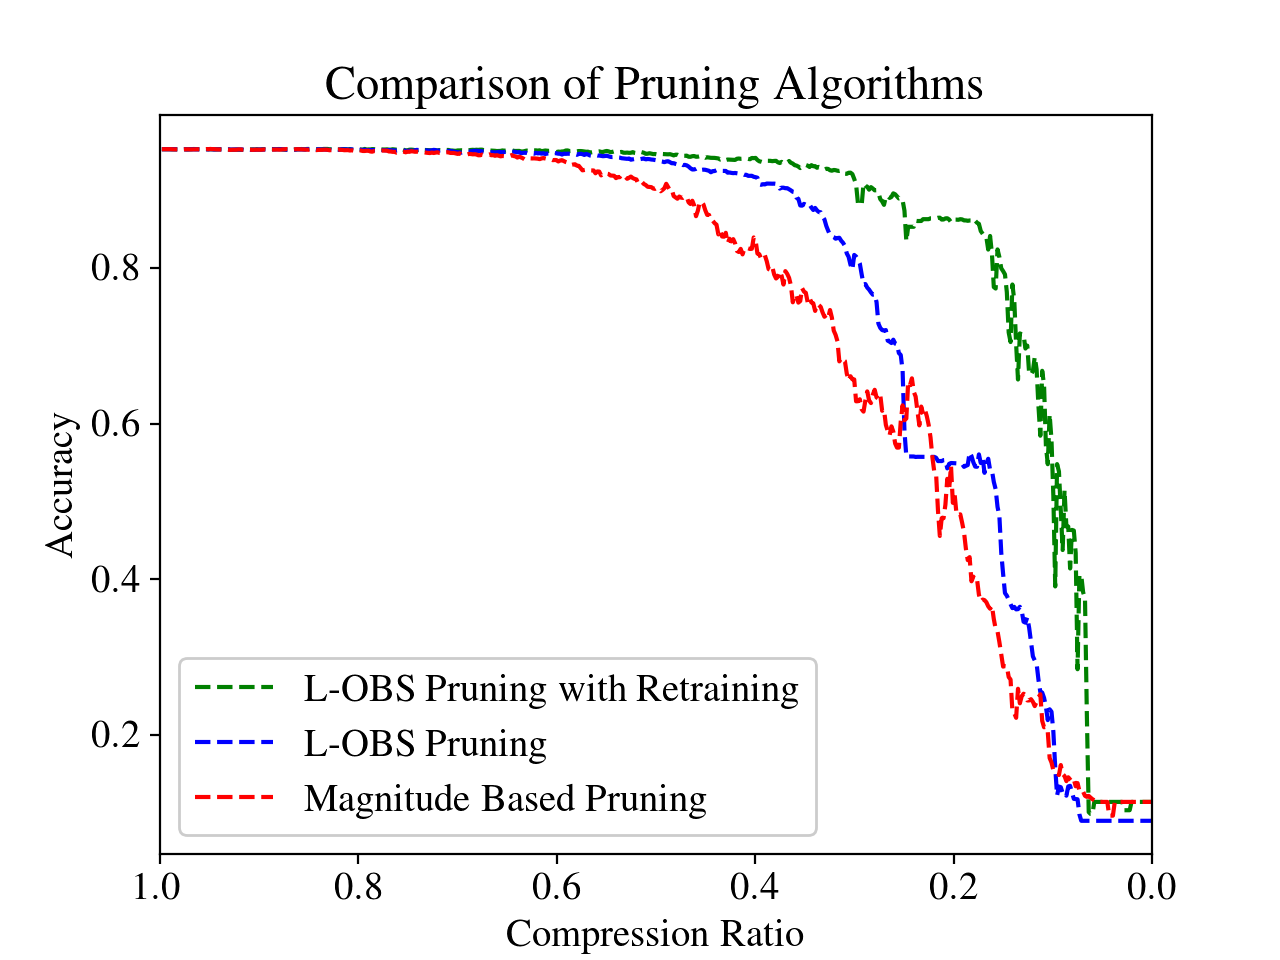
\includegraphics[scale=0.65]{Comparison}

Our control, the Magnitude Based Pruning, dropped in accuracy the fastest, followed by our simplified L-OBS algorithm and then simplified L-OBS with retraining. The L-OBS with retraining graph is particularly jagged, as retraining every 2000 prunings resulted in spikes of accuracy, particularly as the network became more sparse. Interestingly, all algorithms stayed closed to their initial test accuracy until a compression ratio of approximately 0.6. This suggests that the network has redundancies which can be eliminated before training begins.

\section{Future Work}
\label{Future Work}

We hope to combine several of our tested algorithms to see if we can achieve even better compression without loss in accuracy.

You can additionally provide anything else that is relevant to your project but is not present in the list given above. 

You can create various sections/subsections etc. to organize your report as per the need. Use \texttt{biblio.bib} file to provide references. The references should be provided by using cite keyword \cite{langley00}.

You can contact your project mentor if you have any confusion.


%%%%%%%%%%%%%%%%%%%%%%%%%%%%%%%%%%%%%%%%%%%%%%%%%%%%%%%%%%%%%%%%%%%%%%%%%%%%%%%
\newpage

\bibliography{biblio}
\bibliographystyle{icml2018}


%%%%%%%%%%%%%%%%%%%%%%%%%%%%%%%%%%%%%%%%%%%%%%%%%%%%%%%%%%%%%%%%%%%%%%%%%%%%%%%
% Remove this part if you are not using an Appendix. Appendix is ungraded. The
% reader may wish to ignore the appendix altogether. Write everything that you
% think is important in the main report text only.

\appendix
\section{Optional Appendix (Ungraded)}
Remove this part if you are not using an Appendix. Appendix is ungraded. The
reader may wish to ignore the appendix altogether. Write everything that you
think is important in the main report text only.

%%%%%%%%%%%%%%%%%%%%%%%%%%%%%%%%%%%%%%%%%%%%%%%%%%%%%%%%%%%%%%%%%%%%%%%%%%%%%%%

\end{document}